\cotefile{103}
\scanpage{2}\mspage{1}
\margin{\handwritten{9/74\\ Sent by Grothendieck}}

\begin{center}
Sk\deleted{ç}etch of a theory of Gr-Categories\\
by Madame Hoang Xuan Sinh
\end{center}

We give a summary of some results on (Gr)-categories, forming the subject of a detailed work that the author intends to present shortly as a doctoral thesis\handwritten{[\, ]}.

1. Structure of (Gr)-categories.

Our terminology is that of Saavedra \handwritten{[\, ]}. We are interested in categories $C$ equipped with a binary operation $(\deleted{\unsure{x|Y}}X,Y)\handwritten{\mapsto}X\otimes Y$ (func\deleted{\rlap{xxx}\unsure{teu|te}}tor from $C\mathbin{\mathrm{x}}C$ to $C$) associative and unital up to a given isomorphism (satisfying compatibility conditions made explicit in the place cited), also called AU $\otimes$-categories (associative-unital). Such a category is said to be a (Gr)-category if \inserted{\handwritten{it is a groupoid, and if}} every object $X$ of $C$ is ``invertible'', i.e. admits an ``inverse'' object $Y=X^{-1}$ (satisfying $X\otimes Y\handwritten{\simeq}Y\otimes X\handwritten{\simeq}1_C$, where $1_C$ denotes the unit object of $C$). Examples abound:

\uline{Example\handwritten{s}\unsure{.|,}\deleted{1}} \handwritten{1.} $X$ being a topological space\inserted{ pointed at $x\handwritten{\in}X$}, we take for $C$ the category of loop\deleted{\rlap{x}\unsure{s|t}}s in $X$ at $x$, with as morphisms the homotopy classes of homotopies between loops, as operation $\otimes$ the composition of loops (which is not associative, but associative ``up to homotopy'').
% The beginnings of several lines of this left marginal note are clipped by the scan edge.
\margin{\handwritten{\figure{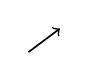
\begin{tikzpicture}[x=1cm,y=1cm]\draw[->,line width=.6pt] (0,0)--(.4,.3);\end{tikzpicture}} \unsure{This|this} example \unsure{is|is} a \unsure{particular} case of the \unsure{following}, by \unsure{taking} $G$ $\unsure{\phantom{=}|=}\Omega^{1}(X,x)$ \unsure{(space} of \unsure{loops}).}}

% The recurring capital below is an overstruck typewriter glyph; its identity remains uncertain.
Variant: $\unsure{\mathbb{G}|G|E|K}$ is an associative Hopf space (or simply homotopy associative in a sufficiently strong sense), $C$ the category whose objects are the points of $\mathbb{G}$, the morphisms the homotopy classes of paths between points of $\mathbb{G}$, the law $\otimes$ being induced by the composition law of $\mathbb{G}$. (NB When $\mathbb{G}$ admits a classifying space $X$, one essentially recovers the preceding example\handwritten{.)}\deleted{\handwritten{which it\unsure{self|selves} \illegible{2}}}

\deleted{\uline{Example}} 2. If $F$ is a sheaf on a topological space (or more generally on a topos), the category $C$ of torsors under $F$, equipped with Baer composition, is a (Gr)-category (and even a strict Picard category, cf. below). One can regard the category $C$ of invertible Modules on a \inserted{\handwritten{locally}} ringed space (or topos) \deleted{\rlap{xxxxx}as} $(X,\underline{O}_{X})$ as the particular case corresponding to the case $F=\underline{O}_{X}^{\handwritten{*}}$.

\deleted{\uline{Example}} 3. If $A$ is a category, the full subcategory \inserted{\handwritten{$C$}} of $\underline{\mathrm{Hom}}(A,A)_{\handwritten{\mathrm{is}}}$ consisting of equivalences of $A$ with itself, equipped with the\deleted{o}\handwritten{'} operation of composition of functors, is a (Gr)-category. Instead of taking for $A$ a category, one can \inserted{\handwritten{more generally}} take for $A$ an object of an arbitrary 2-category. If for example $F$ is a sheaf of groups (not necessarily commutative\deleted{\unsure{s|x}}) on a topological space \handwritten{(}or a topos\handwritten{)}\deleted{$X$}\handwritten{,}
% archive sheet number: 1
